\documentclass[
  bibliography=totoc,     % Literatur im Inhaltsverzeichnis
  captions=tableheading,  % Tabellenüberschriften
  titlepage=firstiscover, % Titelseite ist Deckblatt
]{scrartcl}

% Paket float verbessern
\usepackage{scrhack}

% Warnung, falls nochmal kompiliert werden muss
\usepackage[aux]{rerunfilecheck}

% unverzichtbare Mathe-Befehle
\usepackage{amsmath}
% viele Mathe-Symbole
\usepackage{amssymb}
% Erweiterungen für amsmath
\usepackage{mathtools}

% Fonteinstellungen
\usepackage{fontspec}
% Latin Modern Fonts werden automatisch geladen
% Alternativ zum Beispiel:
%\setromanfont{Libertinus Serif}
%\setsansfont{Libertinus Sans}
%\setmonofont{Libertinus Mono}

% Wenn man andere Schriftarten gesetzt hat,
% sollte man das Seiten-Layout neu berechnen lassen
\recalctypearea{}

% deutsche Spracheinstellungen
\usepackage[ngerman]{babel}


\usepackage[
  math-style=ISO,    % ┐
  bold-style=ISO,    % │
  sans-style=italic, % │ ISO-Standard folgen
  nabla=upright,     % │
  partial=upright,   % │
  mathrm=sym,        % ┘
  warnings-off={           % ┐
    mathtools-colon,       % │ unnötige Warnungen ausschalten
    mathtools-overbracket, % │
  },                       % ┘
]{unicode-math}

% traditionelle Fonts für Mathematik
\setmathfont{Latin Modern Math}
% Alternativ zum Beispiel:
%\setmathfont{Libertinus Math}

\setmathfont{XITS Math}[range={scr, bfscr}]
\setmathfont{XITS Math}[range={cal, bfcal}, StylisticSet=1]

% Zahlen und Einheiten
\usepackage[
  locale=DE,                   % deutsche Einstellungen
  separate-uncertainty=true,   % immer Unsicherheit mit \pm
  per-mode=symbol-or-fraction, % / in inline math, fraction in display math
]{siunitx}

% chemische Formeln
\usepackage[
  version=4,
  math-greek=default, % ┐ mit unicode-math zusammenarbeiten
  text-greek=default, % ┘
]{mhchem}

% richtige Anführungszeichen
\usepackage[autostyle]{csquotes}

% schöne Brüche im Text
\usepackage{xfrac}

% Standardplatzierung für Floats einstellen
\usepackage{float}
\floatplacement{figure}{htbp}
\floatplacement{table}{htbp}

% Floats innerhalb einer Section halten
\usepackage[
  section, % Floats innerhalb der Section halten
  below,   % unterhalb der Section aber auf der selben Seite ist ok
]{placeins}

% Seite drehen für breite Tabellen: landscape Umgebung
\usepackage{pdflscape}

% Captions schöner machen.
\usepackage[
  labelfont=bf,        % Tabelle x: Abbildung y: ist jetzt fett
  font=small,          % Schrift etwas kleiner als Dokument
  width=0.9\textwidth, % maximale Breite einer Caption schmaler
]{caption}
% subfigure, subtable, subref
\usepackage{subcaption}

% Grafiken können eingebunden werden
\usepackage{graphicx}

% schöne Tabellen
\usepackage{tabularray}
\UseTblrLibrary{booktabs, siunitx}

% Verbesserungen am Schriftbild
\usepackage{microtype}

% Literaturverzeichnis
\usepackage[
  backend=biber,
]{biblatex}
% Quellendatenbank
\addbibresource{lit.bib}
\addbibresource{programme.bib}

% Hyperlinks im Dokument
\usepackage[
  german,
  unicode,        % Unicode in PDF-Attributen erlauben
  pdfusetitle,    % Titel, Autoren und Datum als PDF-Attribute
  pdfcreator={},  % ┐ PDF-Attribute säubern
  pdfproducer={}, % ┘
]{hyperref}
% erweiterte Bookmarks im PDF
\usepackage{bookmark}

% Trennung von Wörtern mit Strichen
\usepackage[shortcuts]{extdash}

\author{%
  Vincent Wirsdörfer\\%
  \href{mailto:vincent.wirsdoerfer@udo.edu}{authorA@udo.edu}%
  \and%
  Joris Daus\\%
  \href{mailto:joris.daus@udo.edu}{authorB@udo.edu}%
}
\publishers{TU Dortmund – Fakultät Physik}


\begin{document}
\section{Versuchsdurchführung}

Zu Beginn des Versuchs werden die einzelnen Bestandteile des Oszilloskops sowie des Schwingkreises genauer untersucht 
und auf ihre Funktion überprüft. Im Anschluss soll der effektive Dämpfungswiderstand der Schwingung durch die 
Zeitabhängigkeit der Amplitude berechnet werden. Dazu wird folgende Schaltung aufgebaut:

\begin{figure}
    \centering
    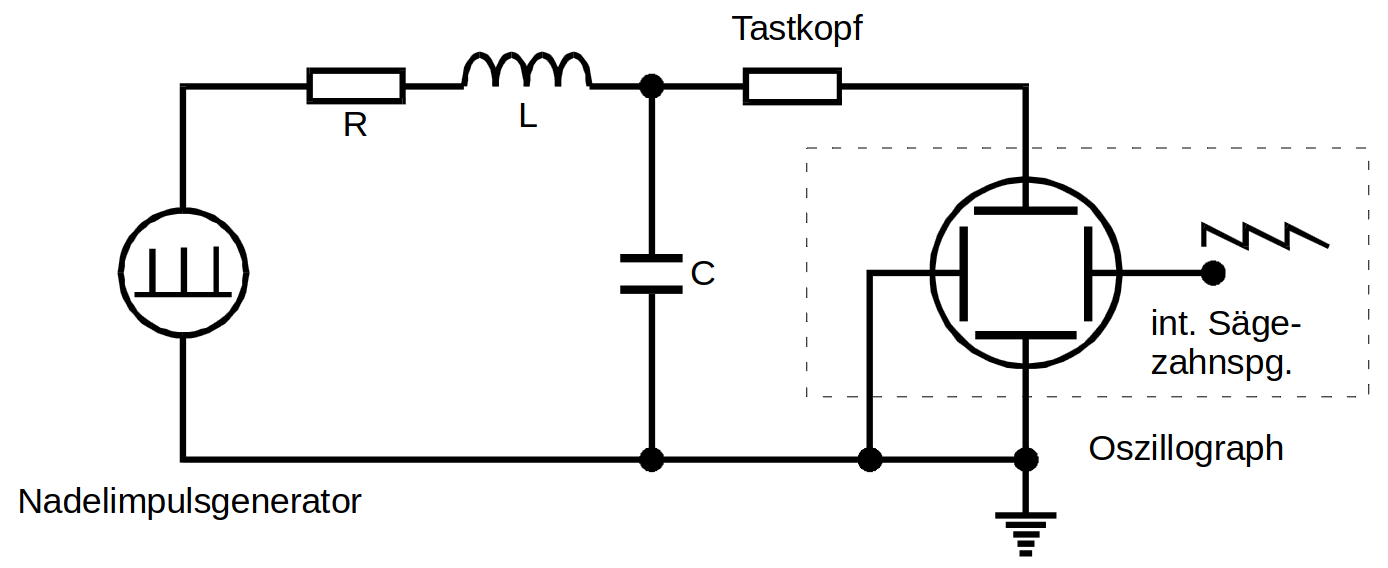
\includegraphics[height=4cm]{5a.png}
    \caption{Schaltung zur Untersuchung des effektiven Dampfungswiderstandes \cite{Versuchsanleitung_v354}.}
    \label{fig:5a}
\end{figure}

\noindent Hierbei ist jedoch zu erwähnen, dass der in Abbildung \ref{fig:5a} zu erkennende Nadelimpulsgenerator \textbf{kein}
Bestandteil des Versuchs ist. Er wird in diesem Fall durch eine Rechteckspannung ersetzt.\\
Auf der digitalen Anzeige des Oszilloskops zeigt sich nun eine gedämpfte Schwingung. Um die zeitliche Abhängigkeit der Amplitude 
zu analysieren werden im Folgenden Wertepaare \{$t$ , $U_\text{C}(t)$\} abgelesen und notiert. Um dieses Bild zu komplettieren 
werden sowohl positive als auch negative Amplituden berücksichtigt.\\\\

\noindent Im nächsten Teilabschnitt des Versuchs soll der der aperiodische Grenzwiderstand $R_\text{ap}$ bestimmt werden. Dazu wird 
die folgende Schaltung aufgebaut:

\begin{figure}[H]
    \centering
    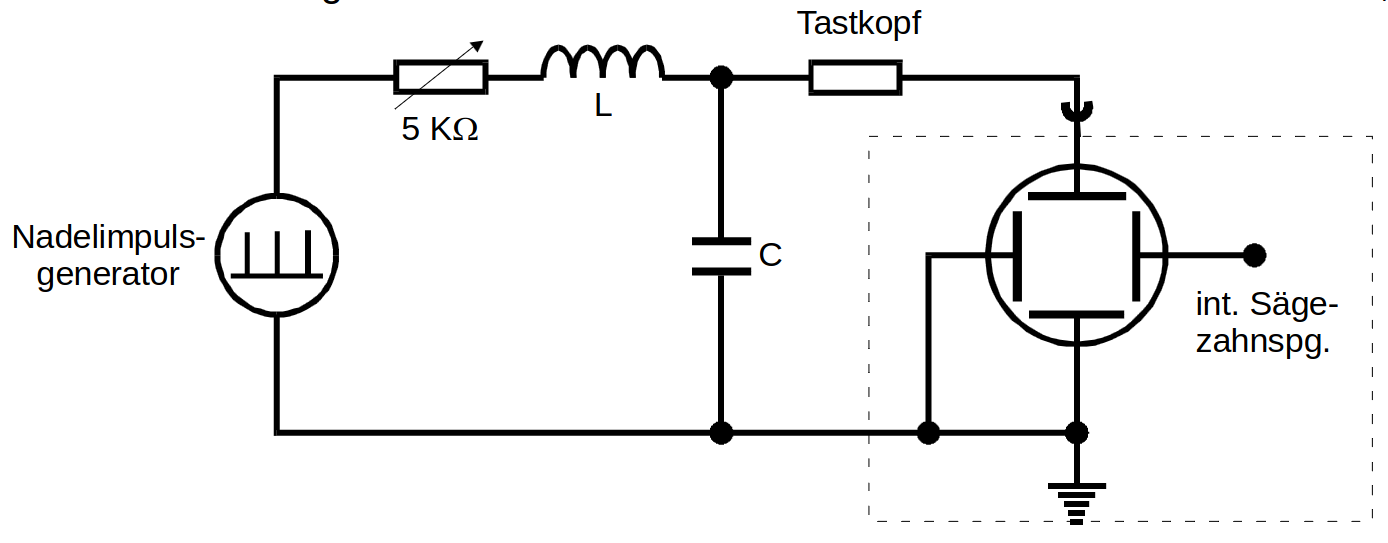
\includegraphics[height=4cm]{5b.png}
    \caption{Schaltung zur Untersuchung des aperiodischen Grenzwiderstandes \cite{Versuchsanleitung_v354}.}
    \label{fig:5b}
\end{figure}

\noindent Zuerst wird der regelbare Widerstand auf sein Maximum gedreht, um ein Relaxationsverhalten (stetige Abnahme der
Kondensatorspannung) zu simulieren. Im Anschluss wird dieser Widerstand behutsam verringert, bis auf der digitalen Anzeige 
des Oszilloskops ein \enquote{Überschwingverhalten} erkennbar ist. Somit ist der aperiodische Grenzwiderstand bereits überschritten.
Dementsprechend muss der Widerstand erneut erhöht werden, sodass das Überschwingverhalten gerade verschwindet. Retrospektiv 
betrachtet wird also versucht, die Abschätzungen aus Gleichung \eqref{eqn:reell} und \eqref{eqn:imaginaer} in die Äquivalenz 
aus Gleichung \eqref{eqn:Grenzfall} zu verwandeln.\\\\

\noindent Im letzen Teil des Versuchs wird die Frequenzabhängigkeit der Kondensatorspannung beobachtet. Die dazu 
benötigte Schaltung wird in der folgenden Abbildung dargestellt.

\begin{figure}[H]
    \centering
    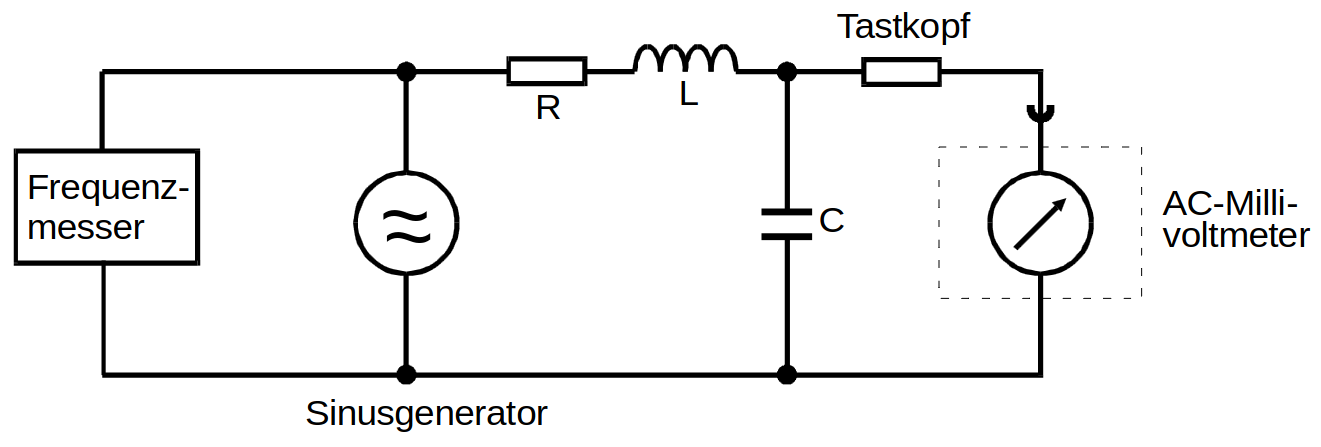
\includegraphics[height=4cm]{5c.png}
    \caption{Schaltung zur Untersuchung des Frequenzabhängigkeit der Kondensatorspannung \cite{Versuchsanleitung_v354}.}
    \label{fig:5c}
\end{figure}

\noindent Zunächst wird die Erregerspannung gemessen. Im Anschluss wird die Frequenz am Sinusgenerator variiert, um 
diverse Wertepare \{$f$ , $U_\text{C}(f)$\}. Diese Datenpaare aus Frequenz und Kondensatorspannung werden letztlich in 
das Heft übertragen.

\section{Messwerte}

\subsection{Zeitabhängigkeit der Amplitude}

Die Untersuchung der Frequenzabhängigkeit der Amplitude zur Bestimmung des effektiven Dämpfungswiderstandes lieftert
folgende Wertepaare:

\begin{table}[H]
    \centering
    \caption{Messdaten zur Bestimmung des effektiven Dämpfungswiderstandes.}
    \sisetup{table-format=1.1}
    \begin{tblr}{
        colspec = {S S S S},
        row{1} = {guard}, row{2} = {guard, mode=math},
    }
    \toprule
    \SetCell[c=2]{c} Positive Amplituden & & \SetCell[c=2]{c} Negative Amplituden & \\
    \cmidrule[lr]{1-2}\cmidrule[lr]{3-4}
    t \mathbin{/} \unit{\second} & U_\text{C} \mathbin{/} \unit{\volt} &  t \mathbin{/} \unit{\second} & U_\text{C} \mathbin{/} \unit{\volt} \\
    \midrule
    5.0e-6  & 3.8 & 1.5e-5  & -3.4 \\
    3.5e-5  & 3.2 & 4.5e-5  & -2.9 \\
    6.5e-5  & 2.7 & 7.5e-5  & -2.4 \\
    9.0e-5  & 2.3 & 1.05e-4 & -2.0 \\
    1.2e-4  & 1.9 & 1.35e-4 & -1.7 \\
    1.5e-4  & 1.6 & 1.65e-4 & -1.4 \\
    1.8e-4  & 1.4 & 1.9e-4  & -1.2 \\
    2.1e-4  & 1.2 & 2.2e-4  & -1.0 \\
    2.4e-4  & 1.0 & 2.6e-4  & -0.9 \\
    2.75e-4 & 0.8 & 2.85e-4 & -0.8 \\
    3.05e-4 & 0.7 & 3.15e-4 & -0.6 \\
    3.3e-4  & 0.6 & 3.45e-4 & -0.6 \\
    3.6e-4  & 0.5 & 3.75e-4 & -0.5 \\
    4.2e-4  & 0.4 & 4.35e-4 & -0.3 \\
    4.8e-4  & 0.3 & 4.95e-4 & -0.2 \\
    \bottomrule
    \end{tblr}
\end{table}

\subsection{Frequenzabhängigkeit der Kondensatorspannung}

Durch die Beobachtung der Frequenzabhängigkeit der Kondensatorspannung werden 
folgende Datenpaare aus Frequenz und Spannung ermittelt:

\begin{table}
    \centering 
    \caption{Messdaten zur Bestimmung der Frequenzabhängigkeit der Kondensatorspannung.}
    \sisetup{table-format=1.1}
    \begin{tblr}{
        colspec = {S[table-format=2.0] S},
        row{1} = {guard, mode=math},
    }
    \toprule
    f \mathbin{/} \unit{\kilo\hertz} & U_\text{C} \mathbin{/} \unit{\volt} \\
    \midrule 
    5  & 2,5  \\
    10 & 2,8  \\
    15 & 3    \\
    20 & 3,6  \\
    22 & 4    \\
    24 & 4,6  \\
    26 & 5,2  \\
    28 & 6,4  \\
    30 & 7,6  \\
    32 & 9    \\
    34 & 9    \\
    36 & 8    \\
    38 & 6,5  \\
    40 & 4,8  \\
    42 & 4    \\
    45 & 2,9  \\
    50 & 2    \\
    \bottomrule
    \end{tblr}
\end{table}

\end{document}

